\documentclass[../main.tex]{subfiles}
\begin{document}
	
	\chapter{Espaços Vetoriais}
	
	\begin{description}
		\item[Videoaula 12 - Espaços Vetoriais] \hfill \\
		\url{https://www.youtube.com/watch?v=UkKQEYRdiks}
		
		\item[Videoaula 18 - Espaços Vetoriais Abstratos] \hfill \\
		\url{https://www.youtube.com/watch?v=dkaUQG1Ic3A}
		
		\item[Videoaula 13 - Subespaços Vetoriais] \hfill \\
		\url{https://www.youtube.com/watch?v=4D-q8OIXa94}
		
		\item[Videoaula 16 - Base e Dimensão] \hfill \\
		\url{https://www.youtube.com/watch?v=wSXwQ3gM7Eo}
		
		\item[Videoaula 17 - Coordenadas] \hfill \\
		\url{https://www.youtube.com/watch?v=GPnZsHawg6A}
		
		\item[Videoaula 20 - Ortogonalidade] \hfill \\ \url{https://www.youtube.com/watch?v=QxsxaQrCHww}
		
		\item[Videoaula 21 - Processo de Ortogonalização de Gram-Schmidt ] \hfill \\
		\url{https://www.youtube.com/watch?v=GbQ-pjpsY9Q}
		
		
	\end{description}
	
	\newpage
	
	Espaços vetoriais são, basicamente, a nossa bancada de trabalho, e os vetores, as ferramentas com as quais construímos muitas funcionalidades. Exemplos disso são as LLMs (ChatGPT, Gemini, DeepSeek) e os sites de busca (Google, DuckDuckGo). Eles utilizam vetores para executar suas tarefas: todas as entradas são convertidas para dentro de um espaço vetorial e, de acordo com a posição do seu vetor, o sistema aproxima os resultados mais relevantes para você.
	
	Além das aplicações na vida real, também temos na matemática pura, espaços vetoriais são muito necessário em cálculo de múltiplas variáveis e uma das bases de análise funcional.
	
	\begin{definicao}
		\azul{Espaços vetorial} é um conjunto $V$ não vazio no qual existe as operações de adição (entre vetores) e multiplicação por um número real (escalar), respeitando as seguintes propriedades com as operações citadas:
		
			\begin{description}
				% O \item[] cria o título da categoria
				\item[Adição:] \hfill 
				\begin{enumerate}
					\item[(A1)] $u + v = v + u$ (Comutatividade)
					\item[(A2)] $(u + v) + w = u + (v + w)$ (Associatividade)
					\item[(A3)] $ \exists v : v + u = u + v = u $ denotamos $v$ por $\vec{0}$ (Vetor nulo)
					\item[(A4)] $\forall u \, \, \exists v : u + v = v + u = \vec{0}$ denotamos $v$ por $-u$ (Inverso aditivo)
				\end{enumerate}
				
				\item[Multiplicação por Escalar:] \hfill 
				\begin{enumerate}
					\item[(M1)] $\alpha(u + v) = \alpha u + \alpha v$ (Distributividade de um escalar)
					\item[(M2)] $(\alpha + \beta)v = \alpha v + \beta v$ (Distributividade de um vetor)
					\item[(M3)] $v \cdot 1 = v$ (Multiplicação por 1)
					\item[(M4)] $\alpha (\beta \cdot v) = (\alpha \cdot \beta)v$ (Associatividade)
				\end{enumerate}
			\end{description}
	\end{definicao}
	\begin{definicao}
		Elementos de um espaço vetorial $V$ são denominados \azul{vetores}.
	\end{definicao}
	\begin{exemplo}[Exemplo de espaço vetorial] O plano euclidiano de dimensão n ($\mathbb{R}^n$) é um dos exemplos mais clássicos de espaço vetorial, seja dois vetores $u=(\eta_1,...,\eta_n)$ e $v=(\delta_1,...,\delta_n)$ e também dois escales $\alpha$ e $\beta$, com sua soma e multiplicação definido por:
	\begin{align*}
		u + v &= (\eta_1 + \delta_1, \dots , \eta_n + \delta_n) \\
		\alpha \cdot u &= (\alpha \eta_1, \dots, \alpha \eta_n)
	\end{align*}
	\begin{center}
		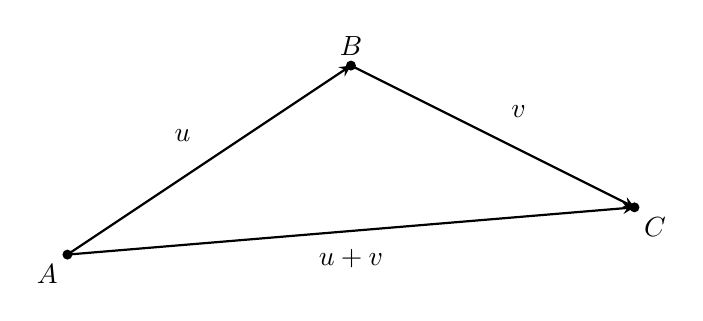
\begin{tikzpicture}[scale=1.2, >=stealth]
			% Pontos
			\coordinate (A) at (0,0);
			\coordinate (B) at (3,2);
			\coordinate (C) at (6,0.5);
			
			% Lados com setas
			\draw[thick, ->] (A) -- (B) node[midway, above left=3pt] {$u$};
			\draw[thick, ->] (B) -- (C) node[midway, above right=3pt] {$v$};
			\draw[thick, ->] (A) -- (C) node[midway, below=3pt] {$u+v$};
			
			% Pontos marcados
			\fill (A) circle (1.5pt) node[below left] {$A$};
			\fill (B) circle (1.5pt) node[above] {$B$};
			\fill (C) circle (1.5pt) node[below right] {$C$};
		\end{tikzpicture}
		(Exemplo no $\mathbb{R}^2$)
		
		
		
		
		
		
		
		
		
		
		
		
		
		
		
		
		
	\end{center}
	
	\end{exemplo}
	\section{Subespaços Vetoriais}
	\section{Base e Coordenadas}
	\section{Ortogonalidade}
		\subsection{Processo de Ortogonalização de Gram-Schmidt}
	
\end{document}
